\begin{figure}[htbp]
\centering 
  \subfloat[Box plot \acs{SCT}.]{
	  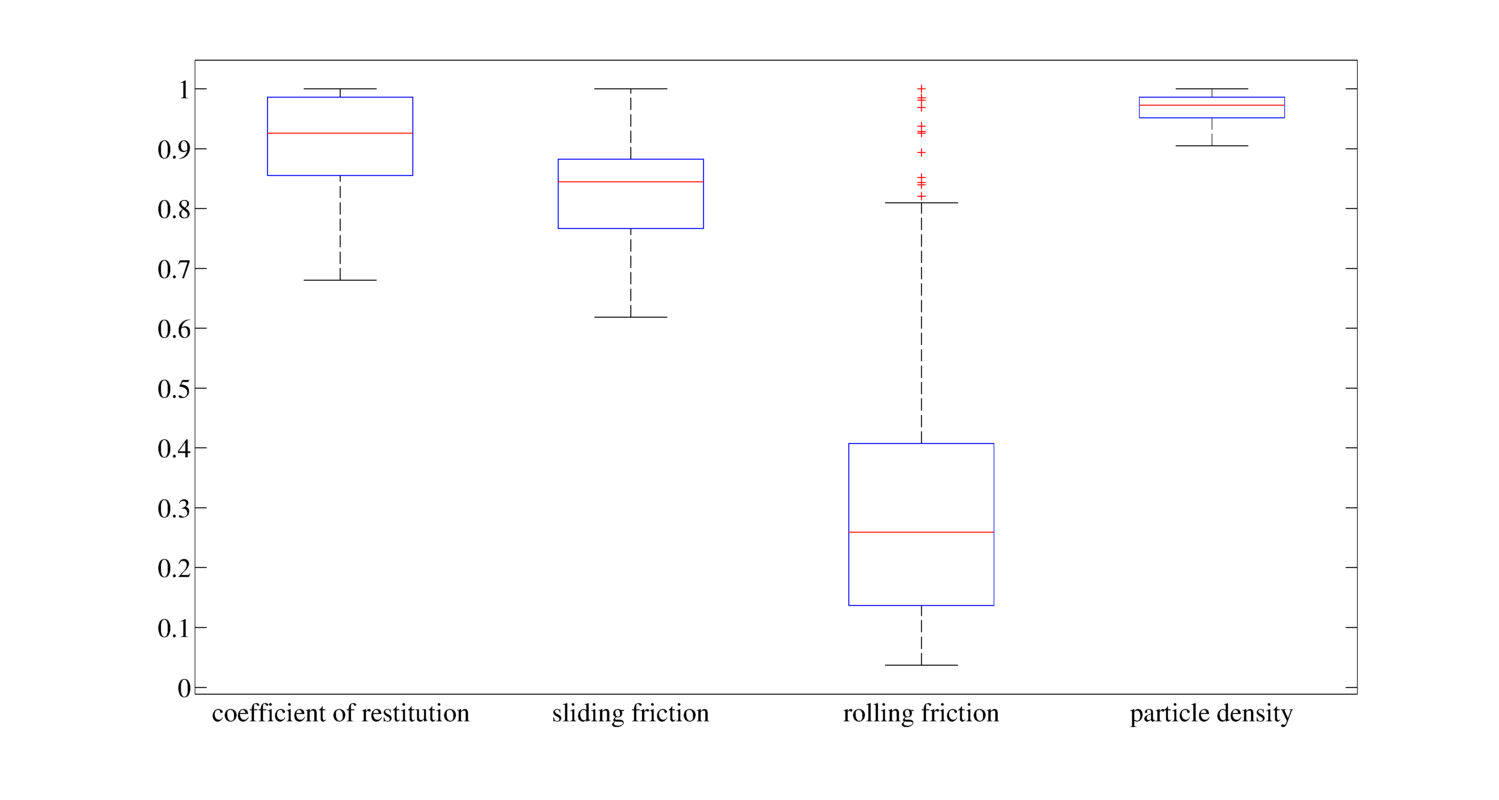
\includegraphics[width=.47\columnwidth]{images/169BoxSCTironorefinetest01coeffP1-20}
	  \label{fig:169BoxSCTironorefinetest01coeffP1-20}
  }
  \quad
  \subfloat[Density plot \acs{SCT}.]{
	  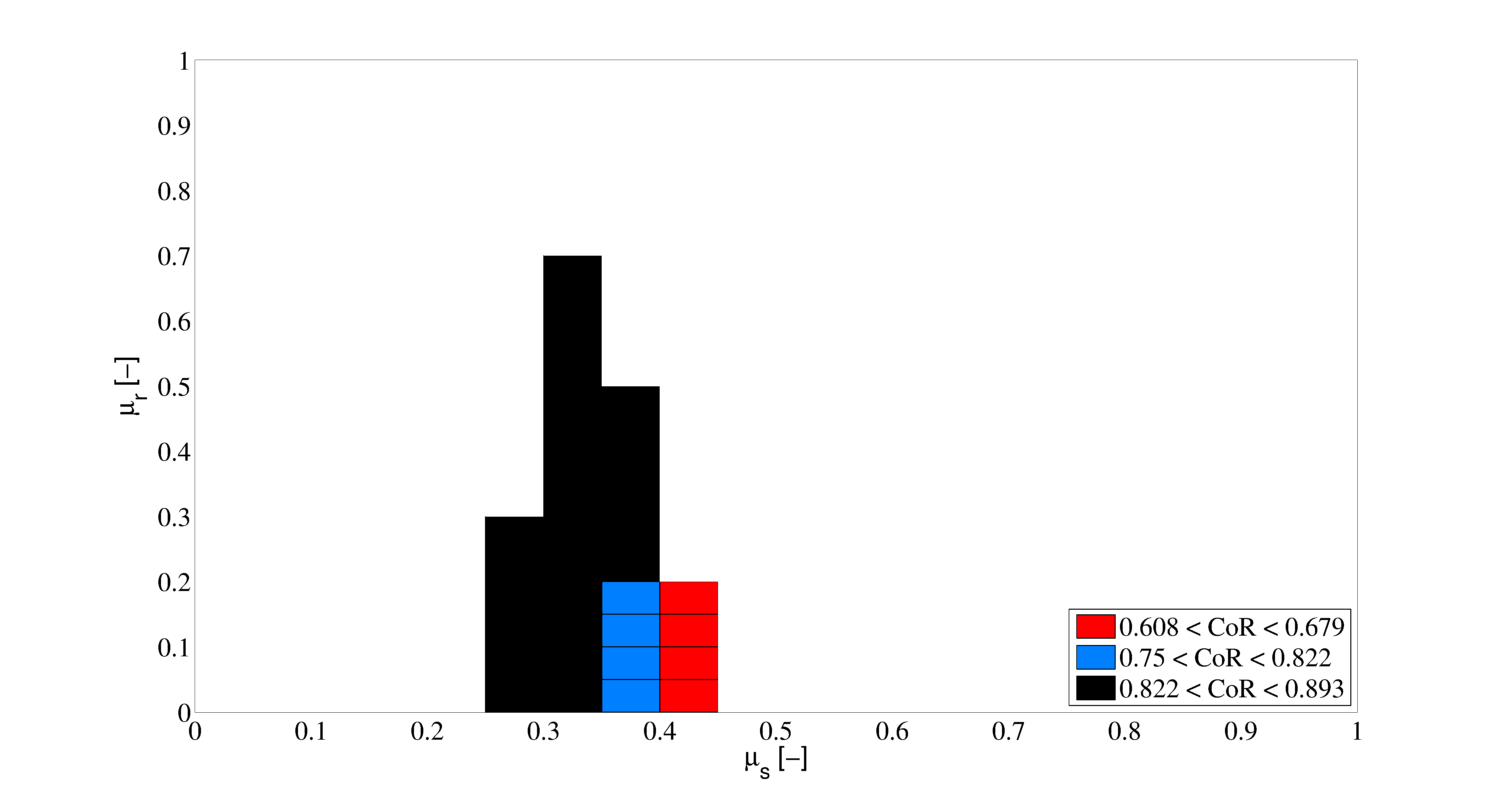
\includegraphics[width=.47\columnwidth]{images/175TileSCironorefinetest01coeffP1}
	  \label{fig:175TileSCironorefinetest01coeffP1}
  }
  \\
    \subfloat[Box plot \acs{AoR}.]{
	  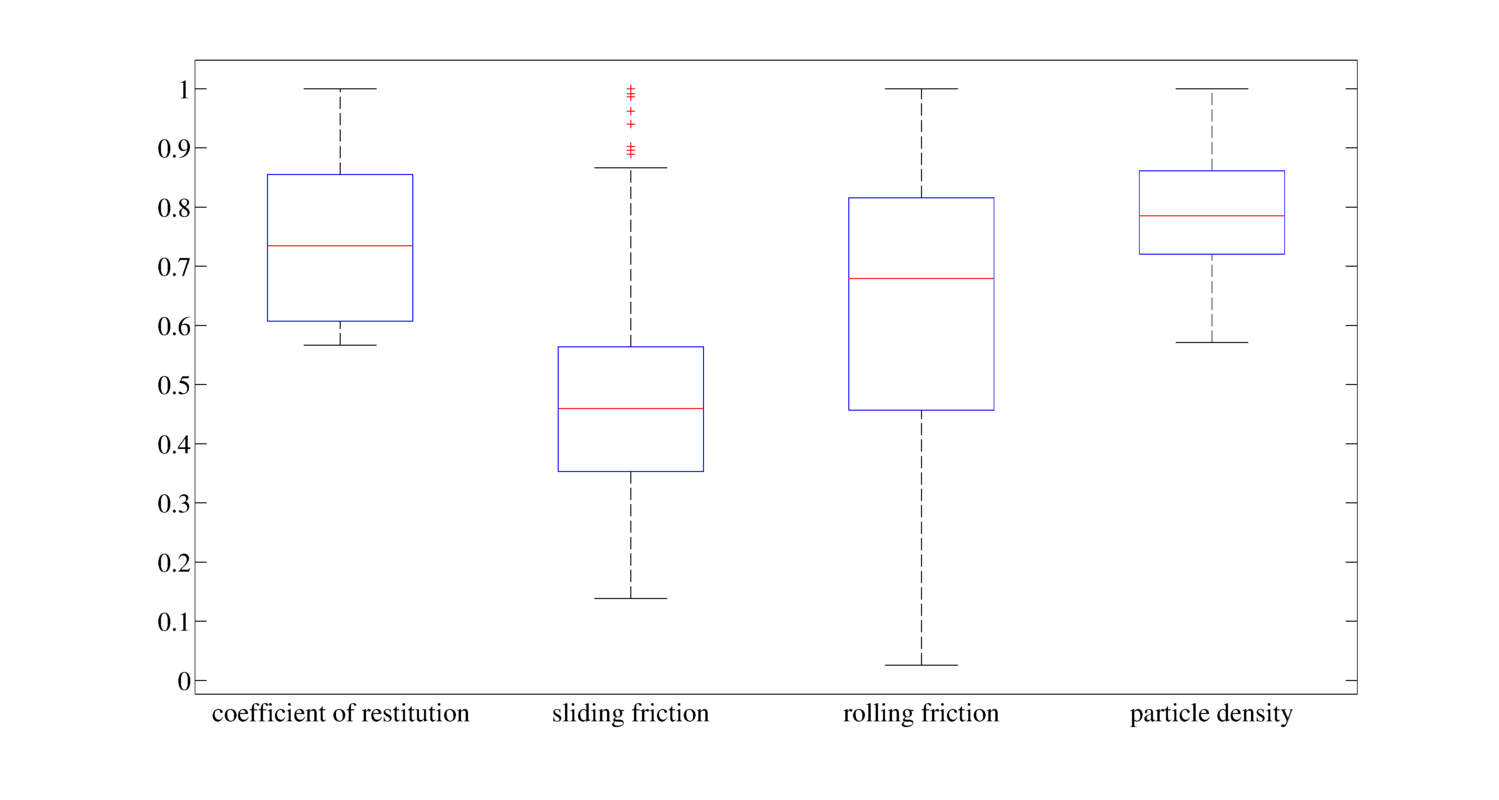
\includegraphics[width=.47\columnwidth]{images/183BoxAORironorefine}
	  \label{fig:183BoxAORironorefine}  }
  \quad
  \subfloat[Density plot \acs{AoR}.]{
	  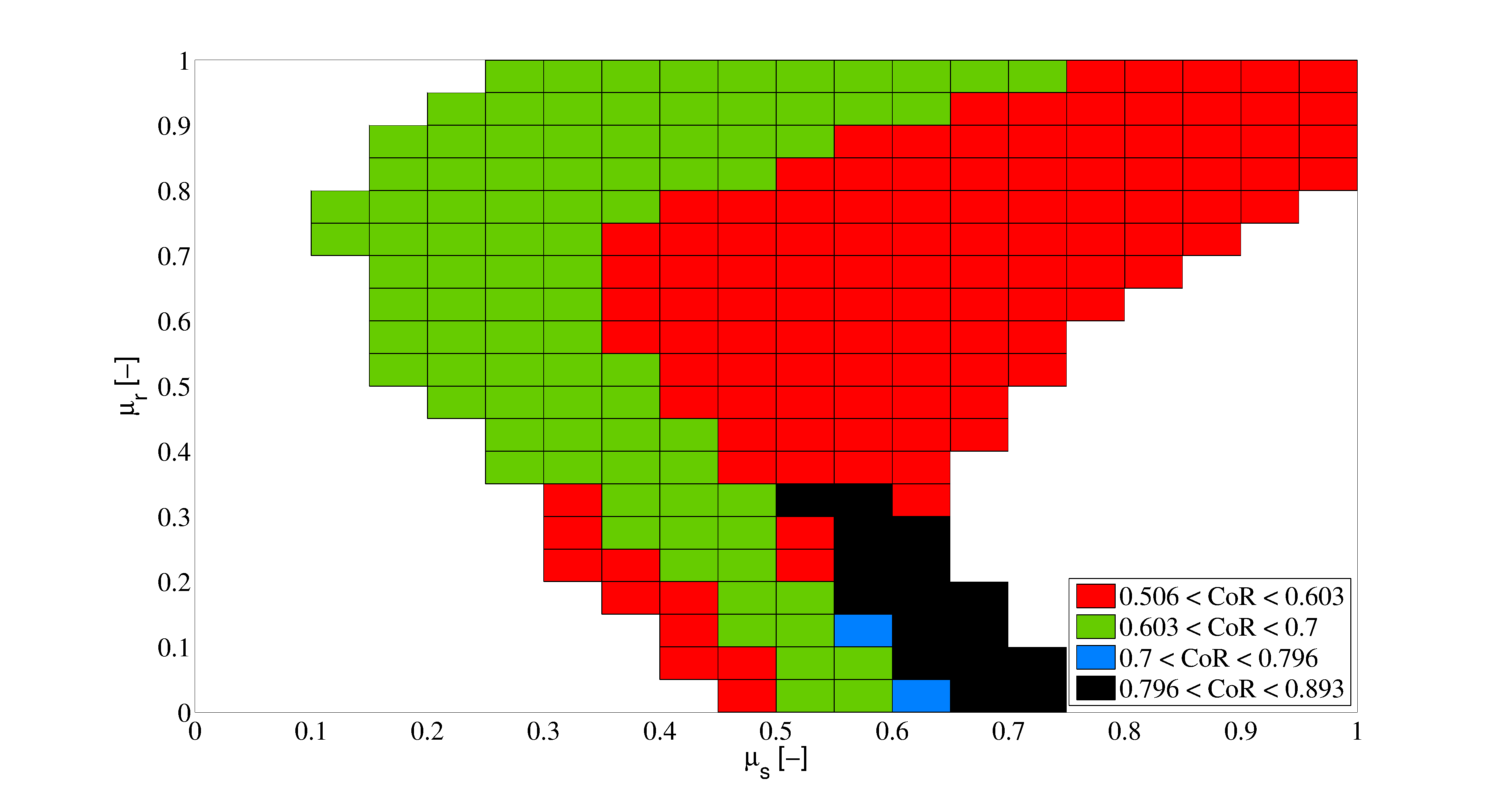
\includegraphics[width=.47\columnwidth]{images/184TileAORironorefine}
	  \label{fig:184TileAORironorefine}  }
  \\
  \subfloat[Box plot intersection: \acs{AoR} \& \acs{SCT}.]{
	  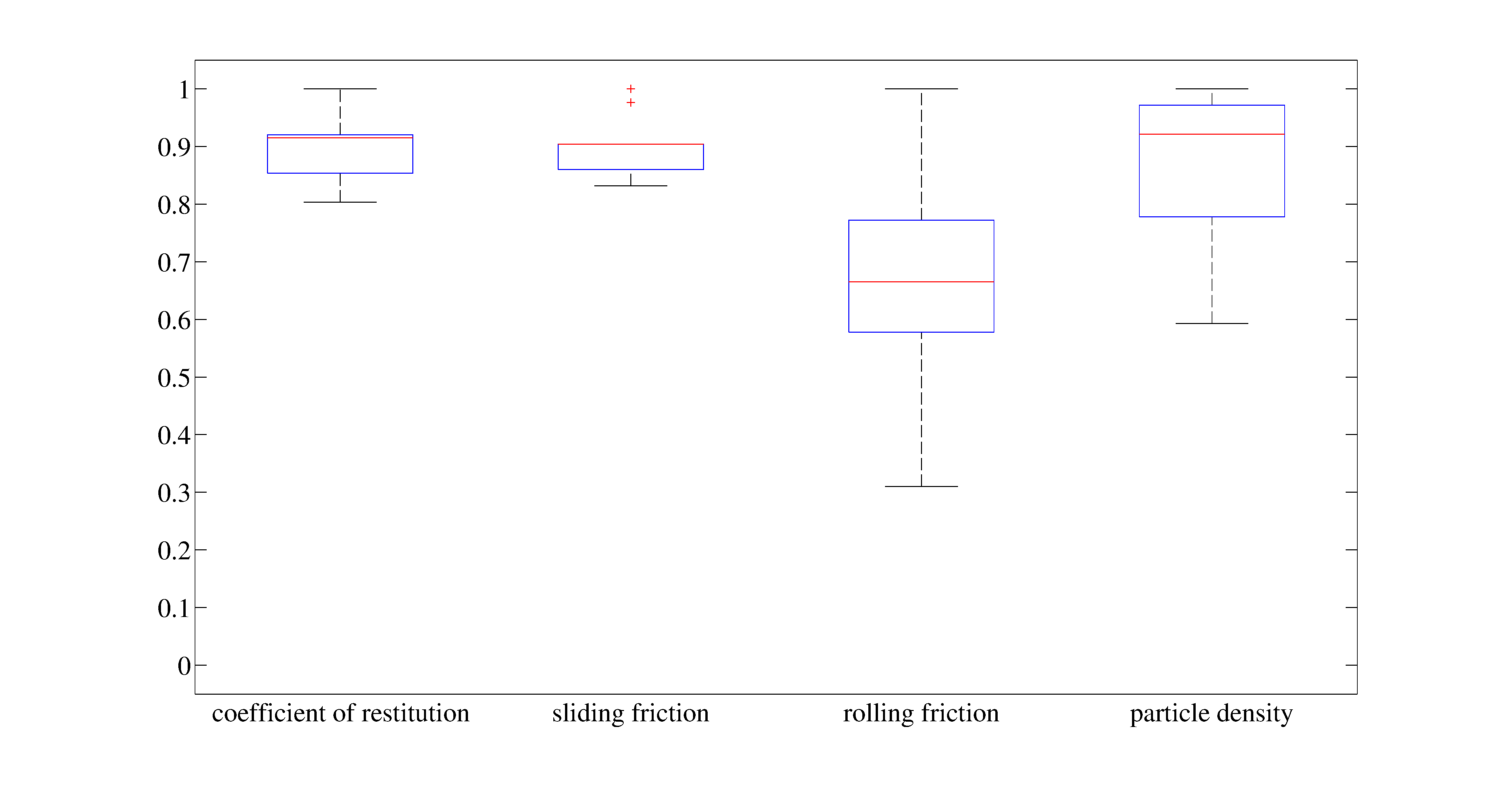
\includegraphics[width=.47\columnwidth]{images/201BoxMixironorefine_30}
	  \label{fig:201BoxMixironorefine_30}
  }
  \quad
  \subfloat[Density plot intersection: \acs{AoR} \& \acs{SCT}.]{
	  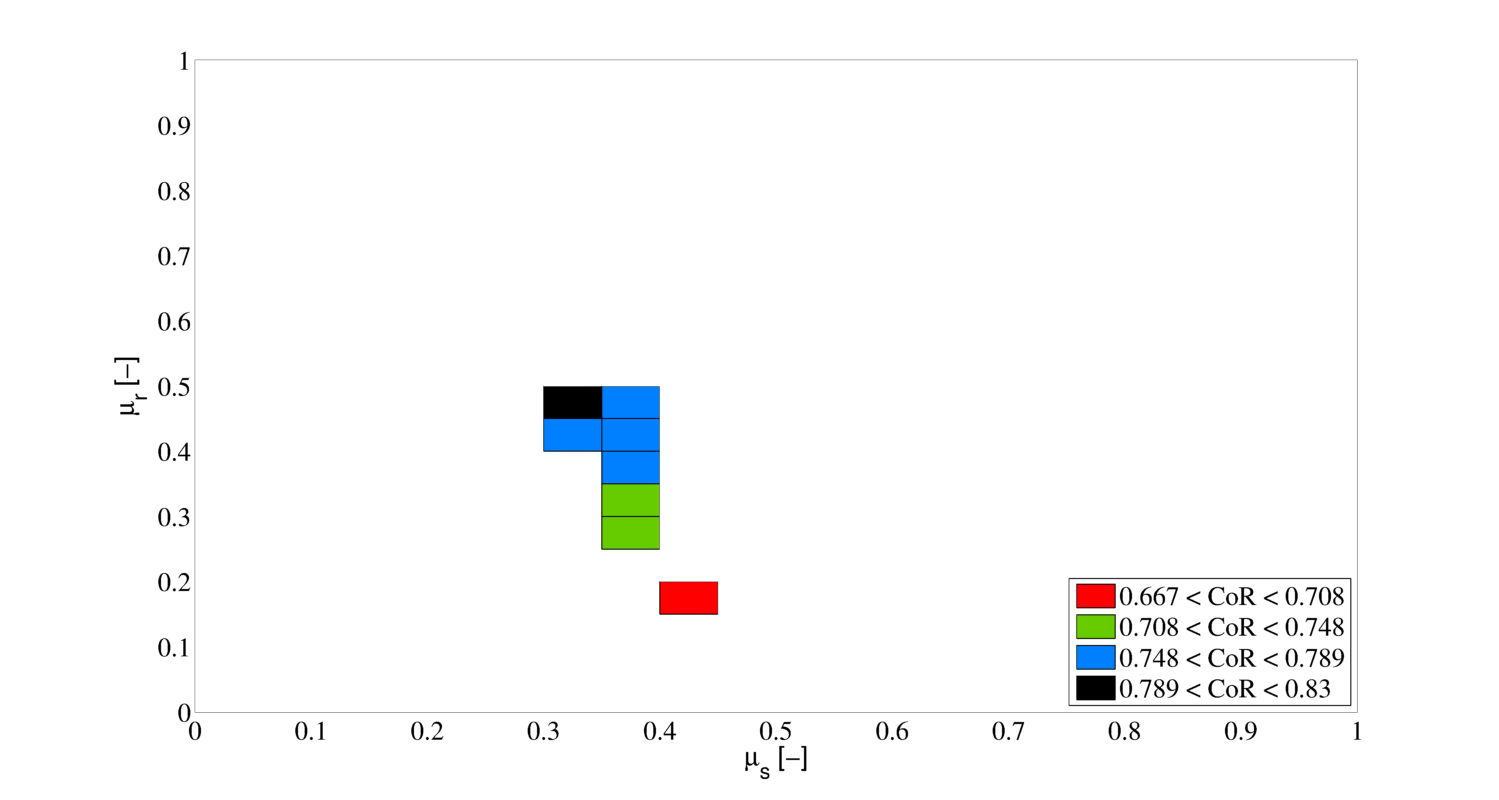
\includegraphics[width=.47\columnwidth]{images/202TileMixironorefine_30}
	  \label{fig:202TileMixironorefine_30}
  }
  \\    
  \caption[Iron ore fine valid values]{Iron ore fine valid values. The valid
  values for the \acs{SCT} and \acs{AoR} tests are shown, together with the merge values, valid for both.
  The plots referring to the single test show reasonably narrow confidence
  ranges, while Fig. \ref{fig:201BoxMixironorefine_30} shows unreasonably large
  valid ranges. See Section \ref{sec:remainingmaterialscharacterization} for
  the interpretation.}
  \label{fig:215boxplotsironorefine}
\end{figure}